\subsubsection{Mandombe-Gruppe}\label{sec:MDB-Gr}

Die Mandombe-Gruppe beschreibt eine keramische Stilgruppe aus dem Gebiet des oberen \mbox{Sangha} sowie \mbox{Ngoko}, deren Formen und Verzierungen am umfangreichsten in Pikunda am \mbox{Sangha} (Fpl.~255) beobachtet wurden. Die an diesem Platz im Grabungsschnitt PIK~87/1 (Kat.-Nr.~8) in Teilen ausgegrabene Grube A enthielt ein umfangreiches keramisches Inventar, das den Grundstock für die Beschreibung der Stilgruppe bildet.\footnote{Da der Name der Fundstelle Pikunda bereits in der Stilgruppe Pikunda-Munda (Kap.~\ref{sec:PKM-Gr}) Verwendung findet und diese Bezeichnung auch in die Literatur eingegangen ist \parencites{Eggert.1992}{Eggert.1993}{Wotzka.1995}, konnte die hier beschriebene Stilgruppe nicht nach jenem Platz benannt werden. In größerem Umfang fand sich auch am Fundplatz Mandombe am \mbox{Sangha} (Fpl.~259) Keramik dieses Stils und dieser wurde daher als eponyme Fundstelle herangezogen.} Diese Grabung sowie vereinzelte Scherben des Mandombe-Stils in der benachbarten, rezenten Grube PIK~87/2 (Kat.-Nr.~9) lieferten insgesamt 508 individuelle GE, die sich der Mandombe-Gruppe zuweisen lassen. 275~GE aus diesen beiden Grabungen wurden individuell aufgenommen und 233 kleinere Scherben ausgezählt erfasst. Vertreter der Mandombe-Gruppe fanden sich auch in den Oberflächenabsammlungen in Pikunda am \mbox{Sangha} sowie am eponymen Fundplatz Mandombe (Fpl.~259). Von diesen und weiteren Funden aus Surveys wurden 92~GE individuell aufgenommen und 51 weitere, kleinere Scherben ausgezählt erfasst. Insgesamt ließen sich GE von 15 Fundstellen der Mandombe-Gruppe zuweisen (Abb.~\ref{fig:MDB_Verbreitung}). Bestimmendes Charakteristikum der Mandombe-Gruppe sind ihre stark bauchigen Kugeltöpfe mit kurzen zylindrischen Hälsen vom Typ D1 und die auf Riefen, Eindrücken und plastischen Elementen basierende Verzierung sowie eine systematische Schlicker-Rauung der Gefäßunterseiten. Das Fundgut der Mandombe-Gruppe setzt sich vornehmlich aus Wandungsstücken zusammen, die 66\,\% aller aufgenommenen Stücke der Stilgruppe ausmachen. Daneben fanden sich etwa 34\,\% Randfragmente und nur zwei hinreichend vollständige Gefäße (Abb.~\ref{fig:MDB_Typverteter}.1; Taf.~48.2).

\begin{figure*}[!tb]
	\centering
	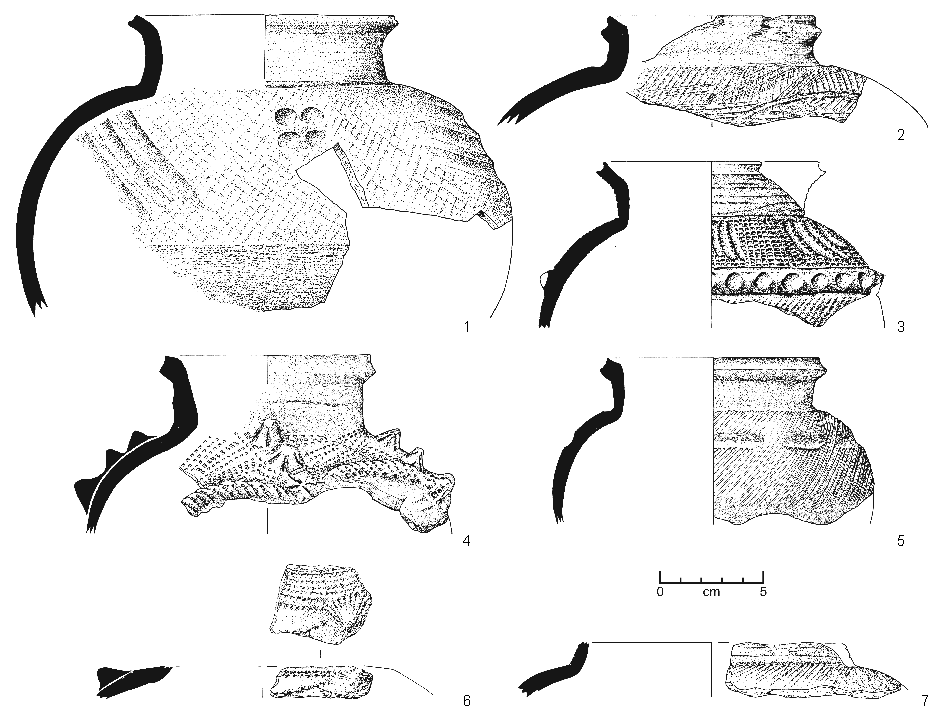
\includegraphics[width=\textwidth]{fig/MDB-Typen.pdf}
	\caption{Mandombe-Gruppe: Typvertreter.\\1:~Taf.~47.24; 2:~Taf.~48.4; 3:~Taf.~55.11; 4:~Taf.~47.23; 5:~Taf.~47.22; 6:~Taf.~57.11; 7:~Taf.~62.6.}
	\label{fig:MDB_Typverteter}
\end{figure*}

\begin{figure*}[!tb]
	\centering
	\begin{subfigure}[t]{.32\textwidth}
		\centering
		
\includegraphics[width = \textwidth, page = 1]{tbl/Tab_Fabrics/x_fabrics_scales.pdf}
		\includegraphics[width = \textwidth]{tbl/Tab_Fabrics/PIK87-2-6-77_outer_5cm.jpg}
		\caption{Außenseite.}
		\label{fig:PIK87-2-6-77_aussen}
	\end{subfigure}\hfill
	\begin{subfigure}[t]{.32\textwidth}
		\centering
		
\includegraphics[width = \textwidth, page = 2]{tbl/Tab_Fabrics/x_fabrics_scales.pdf}
		\includegraphics[width = \textwidth]{tbl/Tab_Fabrics/PIK87-2-6-77_2cm.jpg}
		\caption{Profil.}
		\label{fig:PIK87-2-6-77_profil}
	\end{subfigure}\hfill
	\begin{subfigure}[t]{.32\textwidth}
		\centering
		
\includegraphics[width = \textwidth, page = 1]{tbl/Tab_Fabrics/x_fabrics_scales.pdf}
		\includegraphics[width = \textwidth]{tbl/Tab_Fabrics/PIK87-2-6-77_inner_5cm.jpg}
		\caption{Innenseite.}
		\label{fig:PIK87-2-6-77_innen}
	\end{subfigure} %
	\caption{Mandombe-Gruppe: Scherbe eines aus einem weißbrennenden Ton getöpfertes Gefäß mit innenseitig aus rotbrennendem Ton bestehendem Schlicker (\textbf{B}--\textbf{C}; Kat.-Nr.~9).}
	\label{fig:PIK87-2-6-77}
\end{figure*}

\paragraph{Technologische Merkmale}\hspace{-.5em}|\hspace{.5em}%
Mandombe-Keramik zeichnet sich durch hohe Anteile nichtplastischer Partikel aus. 68\,\% aller GE weisen mehr als 15--20\,\% nichtplastische Partikel im Scherben auf, die vornehmlich den Größenklassen \textit{medium} (33\,\%) bis \textit{coarse} (55\,\%) zuzurechnen sind. Es handelt sich größtenteils (60\,\%) um feinen, heterogenen Quarzsand sowie ausgebrannte Organik (siehe Abb.~\ref{PIK87-1-2-3_1-3-7_Makrospuren}). Selten finden sich auch Glimmer oder lateritähnliche Partikel. Zusammengenommen 88\,\% der Scherben lassen sich einem \textit{Fabric} der Gruppe 3 zuweisen, wobei 50\,\% auf die Variante 3a, 26\,\% auf die Variante 3b und 3\,\% auf die Variante 3c entfallen. Weitere 21\,\% ließen sich nicht genau einer Variante zuordnen.\footnote{Auch die bei ihrer Herstellung 1987 in Pikunda beobachteten Gefäße weisen einen Scherben auf, der dem \textit{Fabric} 3 entspricht. Damit lassen sich Rückschlüsse auf Rohmaterialgewinnung und Rohmaterialaufbereitung sowie den Brand der Gefäße der Mandombe-Gruppe ziehen. Siehe Anm.~\ref{ftn:EthnoToepfereiInVorb}.} Neben \textit{Fabrics} des Typs 3 finden sich in sehr geringen Anteilen Stücke, die einzelnen Varietäten der \textit{Fabrics} 4--8 zuordenbar sind. Die Brennfarbe lässt sich, aufgrund grauer bis beiger Farbtöne, für etwa 45\,\% aller Stücke nicht hinreichend genau bestimmen. Stücke, deren Färbung auf die Nutzung rotbrennender Tone hindeuten, machen 31\,\% aus, während solche, die weißbrennende Tone anzeigen, etwa 23\,\% ausmachen. Die Oberflächen der Stücke sind geglättet (69\,\%) oder leicht rau (22\,\%). Die Dicke der Gefäßwandungen liegt im arithmetischen Mittel bei 6,9\,mm, mit einer Varianz von 3,7\,mm.

Charakteristisch ist der zwar hohe Anteil nichtplastischer Partikel, jedoch auch die Begrenzung auf Partikel der Größenklassen \textit{medium} bis \textit{coarse}. Gerade innerhalb einer GE schwankt die Korngröße der nichtplastischen Partikel nur wenig und man gewinnt den Eindruck, das Korngrößenspektrum sei künstlich eingegrenzt worden, zum Beispiel durch Sieben. Die zweite wichtige technische Eigenheit der Mandombe-Keramik betrifft die beobachtbaren Auswirkungen des Brandes auf die Färbung der Stücke. Fast alle Stücke, wiederum auch ein bestimmendes Merkmal der \textit{Fabrics} vom Typ 3, zeigen lediglich eine randliche, deutlich von einem homogen grauen Kern abgegrenzte Oxidation (Abb.~\ref{fig:PIK87-2-6-77_profil}).\footnote{Neben diesen Charakteristika der Mandombe-Keramik fand sich im Fundgut der rezenten Grube PIK~87/2 in Pikunda am \mbox{Sangha} (Kat.-Nr.~9; Fpl.~255) eine GE, die auf ihrer Innenseite einen zusätzlichen Auftrag aufweist. Das aus weißbrennendem Ton aufgebaute Gefäß zeigt innen eine deutlich abgrenzbare, rote Lage (Abb.~\ref{fig:PIK87-2-6-77}).}

\begin{figure*}[p]
	\centering
	\includegraphics[width=\textwidth]{fig/MDB_Verbreitung.pdf}
	\caption{Mandombe-Gruppe: Verbreitung \parencite[P1 nach][114 Abb.~42]{Gillet.2013}.}
	\label{fig:MDB_Verbreitung}
\end{figure*}

\paragraph{Formen}\hspace{-.5em}|\hspace{.5em}%
Das Formenspektrum der Mandombe-Gruppe ist sehr homogen. Während bei insgesamt 119~GE die Gefäßform angesprochen werden konnte, war die Bestimmung nur bei etwas über der Hälfte dieser Stücke hinreichend zuverlässig möglich. Insgesamt 87\,\% aller Formen machen Gefäße mit stark konvexer Wandung und ohne ausgeprägten Halsbereich aus (Abb.~\ref{fig:MDB_Typverteter}), wobei sichere und fragliche Ansprachen zu etwa gleichen Teilen vorkommen.\footnote{Die maximalen Durchmesser dieser Gefäße schwanken zwischen zwölf und 32\,cm. Die aufgenommenen Durchmesser an den verschiedenen Gefäßpositionen wie Mündung, minimaler Halsdurchmesser sowie maximaler Bauchdurchmesser (Abb.~\ref{fig:GefAbmessungen_Schema}) zeigen jeweils mehr oder weniger eingipfelige Verteilungen und lassen keine konkreten Größenklassen erkennen, die eine weitere Untergliederung rechtfertigen könnten. Während die Messungen der Durchmesser an der Gefäßmündung sowie der minimale Durchmesser im Halsbereich jeweils einer eingipfeligen Normalverteilung entspricht, streut die Verteilung für den maximalen Bauchdurchmesser stärker. Die Höhen der Mündung (Abb.~\ref{fig:GefAbmessungen_Schema}) konnten -- da kein Gefäß hinreichend erhalten war -- bei keiner GE ermittelt werden. Rekonstruiert man jedoch die stark kugelige Form der Gefäße und projiziert entsprechend runde Böden, so müssten die Höhen der Gefäße in etwa bei Werten um die entsprechenden maximalen Durchmesser gelegen haben.} Das Spektrum an Randformen der Mandombe-Gruppe wird von ausbiegenden Rändern bestimmt. Das Gros bilden kurze, einfach ausbiegende Formen vom Typ B1.1. Diese machen knapp die Hälfte aller 120 aufgenommenen Ränder aus. Zahlreich kommen noch konkav (B2; 29\,\%) sowie gerade ausbiegende Ränder (B1; 12\,\%) vor. Die Randlippen weisen regelhaft eine Rille auf (M4; 90\,\%; Abb.~\ref{fig:MDB_Typverteter}.1--5). Die Halspartien der Gefäße sind zu 91\,\% kurz und überwiegend zylindrisch (31\,\%) oder konkav (33\,\%) ausgeführt. In einigen Fällen verläuft auf dem Gefäßhals ein horizontaler Wulst (Abb.~\ref{fig:MDB_Typverteter}.2, 4). Die Gefäßschultern sind überwiegend deutlich konvex (72\,\%). Die Ausprägung des Gefäßbodens konnte bei keiner der sicher der Mandombe-Gruppe zugerechneten GE beobachtet werden. Zwei nicht zweifelsfrei der Stilgruppe zugehörige GE zeigen runde Böden (B1--B2), während drei weitere Stücke auf flache (B4) oder profiliert abgesetzte Flachböden (B9--10) hindeuten. Eine spezifische Bodenform ließ sich der Mandombe-Gruppe nicht zuweisen.

\paragraph{Verzierungen}\hspace{-.5em}|\hspace{.5em}%
Das Spektrum an Verzierungen innerhalb der Mandombe-Gruppe wird von diagonalem (Tab.~\ref{tab:Verzierungselemente}: 15.1; 21\,\%) oder überkreuztem Kammstrich (Tab.~\ref{tab:Verzierungselemente}: 15.2; 8\,\%), mehr als 5\,mm breite Riefen (Tab.~\ref{tab:Verzierungselemente}: 02.7; 14\,\%) sowie einfachen horizontalen Riefen (Tab.~\ref{tab:Verzierungselemente}: 02.1; 14\,\%) bestimmt. Der Kammstrich besteht häufig aus Riefen mit kantigem, u-förmigem Profil und findet sich vornehmlich im Schulterbereich sowie auf dem Gefäßbauch (Anlage~4\subref{fig:MDB_Verz}). Auch die breiten Riefen finden sich vornehmlich in diesen beiden Gefäßregionen, während die horizontalen Rillen größtenteils im Hals- sowie Schulterbereich der Gefäße beobachtet wurden. Seltener, jedoch um so charakteristischer sind plastische Elemente wie Knubben (Tab.~\ref{tab:Verzierungselemente}: 09.1; 6\,\%) und Leisten (Tab.~\ref{tab:Verzierungselemente}: 09.2; 2\,\%). Auch sie sind vornehmlich auf dem Schulterbereich der Gefäße zu finden. Die Gefäßunterseiten sind regelhaft unverziert, weisen aber, sofern diese Partie erhalten ist, häufig eine Schlicker-Rauung auf (Abb.~\ref{fig:MDB_Typverteter}.1). Grundsätzlich finden sich über die Hälfte aller aufgenommenen Verzierungselemente (55\,\%) im Bereich der Gefäßschulter, gefolgt vom Bauchbereich (27\,\%). Die Ränder sind innen wie außen nur selten verziert, ähnlich der Gefäßhälse.

Lediglich drei zweifelsfrei der Mandombe-Gruppe zuordenbare Randscherben aus dem Survey in Pikunda am \mbox{Sangha} (Fpl.~255) weisen \textit{knotted string}-\mbox{Roulette} (Tab.~\ref{tab:Verzierungselemente}: 21.1) im Schulterbereich auf. In allen Fällen wird das \mbox{Roulette} von breiten Reifen überlagert (Taf.~55.12) sowie von Knubben oder plastischen Leisten begleitet. Die starke Ähnlichkeiten zur Mandombe-Keramik aufweisende Konda-Gruppe (Kap.~\ref{sec:KON-Gr}) zeigt ebenfalls ein auf Einzelstücke begrenztes Auftreten von Rouletteverzierung.

\paragraph{Datierung}\hspace{-.5em}|\hspace{.5em}%
Für die Keramik der Mandombe-Gruppe liegt eine Radiokohlenstoffdatierung aus der im Grabungsschnitt PIK~87/1 (Kat.-Nr.~8) in Pikunda am \mbox{Sangha} (Fpl.~255) erfassten Grube A vor. Sie datiert demnach in das 13.--15.~Jh. n.~Chr. (Tab.~\ref{tab:PIK87-1_Datierungen}: KI-2891).\footnote{Die benachbarte Grube PIK~87/2 (Kat.-Nr.~9) enthielt ebenfalls keramisches Material, welches der Mandombe-Gruppe zugerechnet beziehungsweise nicht sicher abgegrenzt werden kann. Grundsätzlich muss der Befund jedoch als rezent angesehen werden, wie der Fund eines Plastik-Kamms zeigt. Die Mandombe-Keramik ist mit hoher Wahrscheinlichkeit mit dem Verfüllungsmaterial in die rezente Grube gelangt. Auffällig ist, dass die entsprechende Keramik aus dem Befund PIK~87/2 Rouletteverzierung aufweist, sich ansonsten aber nicht vom Material der Grube A in PIK~87/1 unterscheidet. Ob dies eine sukzessive Integration von Rouletteverzierung in das Verzierungs-Spektrum der Mandombe-Gruppe anzeigt, muss beim gegenwärtigen Stand der Feldarbeiten offenbleiben.}

\paragraph{Verbreitung}\hspace{-.5em}|\hspace{.5em}%
Keramik der Mandombe-Gruppe findet sich fast ausschließlich im Bereich des oberen \mbox{Sangha} sowie an zwei Fundstellen entlang des \mbox{Ngoko} (Abb.~\ref{fig:MDB_Verbreitung}).\footnote{Potenziell der Mandombe-Gruppe zurechenbare Stücke wurden auch in Mboua Mboua am oberen \mbox{Sangha} gefunden \parencite[114 Abb.~42]{Gillet.2013}. Siehe auch Kap.~\ref{sec:PKM-Gr}.} Der südlichste Fundpunkt der Verbreitung und die mit Blick auf die absolut vorliegenden Fundanteile bestimmende Fundstelle ist Pikunda am mittleren \mbox{Sangha} (Fpl.~255). Im Norden, stromauf des \mbox{Sangha}, sowie möglicherweise entlang des \mbox{Ngoko} im Westen, ist die Grenze des Verbreitungsgebietes der Mandombe-Gruppe nicht erfasst und wird lediglich durch die Grenzen des Arbeitsgebietes bestimmt. Gerade die ungleiche Verteilung von aus Pikunda stammenden Grabungsfunden gegenüber deutlich selteneren Surveyfunden erschwert eine stichhaltige Interpretation des Verbreitungsgebietes der Mandombe-Keramik. 